\documentclass[twoside]{article}
\usepackage{mdframed}
\usepackage[hmarginratio=1:1,top=32mm,columnsep=20pt]{geometry} % Document margins
\usepackage{multicol} % Used for the two-column layout of the document
\usepackage[hang, small,labelfont=bf,up,textfont=it,up]{caption} % Custom captions under/above floats in tables or figures
\usepackage{booktabs} % Horizontal rules in tables
\usepackage{float} % Required for tables and figures in the multi-column environment - they need to be placed in specific locations with the [H] (e.g. \begin{table}[H])
\usepackage{hyperref} % For hyperlinks in the PDF
\usepackage{amsmath,amsthm,amssymb}
\usepackage{lettrine} % The lettrine is the first enlarged letter at the beginning of the text
\usepackage{paralist} % Used for the compactitem environment which makes bullet points with less space between them
\usepackage{tikz}
\usepackage{esint}
\usepackage{centernot}
\usepackage{lmodern}
\usetikzlibrary{3d}
\usetikzlibrary{patterns,calc,hobby}
\usetikzlibrary{decorations.pathreplacing}
\tikzset{
	partial ellipse/.style args={#1:#2:#3}{
		insert path={+ (#1:#3) arc (#1:#2:#3)}
	}
}
\usepackage{xcolor}

\usepackage{fancyhdr} % Headers and footers
\pagestyle{fancy} % All pages have headers and footers
\fancyhead{} % Blank out the default header
\fancyfoot{} % Blank out the default footer
\fancyhead[C]{Jimmy Yue $\bullet$ Statistics $\bullet$ Jimmy Yue} % Custom header text
\fancyfoot[RO,LE]{\thepage} % Custom footer text

\newmdenv[skipabove=7pt,
rightline=false,
leftline=true,
topline=false,
bottomline=false,
skipbelow=5pt,
linecolor=black,
innerleftmargin=5pt,
innerrightmargin=5pt,
innertopmargin=5pt,
leftmargin=0cm,
rightmargin=0cm,
linewidth=4pt,
innerbottommargin=5pt]{cBox}

\theoremstyle{definition}
\newtheorem*{solutionT}{Solution}

\newenvironment{solution}{\begin{cBox}\begin{solutionT}}{\hfill{\scriptsize\ensuremath{\square}}\end{solutionT}\end{cBox}}

%%%%%%%%%%%%%%%%%%%%%%%%%%%%%%%%%%%%%%%%%%%%%%%%%%%%%%%%%%%%%%%%%%%%%%%%%%%%%%%%%%%%%%%%%%%%
\newcommand{\vect}[1]{\vec{\pmb{#1}}}
\newcommand{\uvect}[1]{\hat{\mathbf{#1}}}
\newcommand{\leviciv}{\epsilon_{ijk}}

\newmdenv[skipabove=7pt,
rightline=false,
leftline=true,
topline=false,
bottomline=false,
skipbelow=5pt,
linecolor=black,
innerleftmargin=5pt,
innerrightmargin=5pt,
innertopmargin=5pt,
leftmargin=0cm,
rightmargin=0cm,
linewidth=4pt,
innerbottommargin=7,
backgroundcolor=light-gray]{dBox}



\theoremstyle{definition}
\newtheorem*{proof1}{Definition}

\newenvironment{ddef}{\begin{dBox}\begin{proof1}}{\hfill{\scriptsize}\end{proof1}\end{dBox}}
\newcommand{\pdif}[2]{\frac{\partial#1}{\partial#2}}
\definecolor{light-gray}{gray}{0.85}
%----------------------------------------------------------------------------------------
%-	TITLE SECTION
%----------------------------------------------------------------------------------------

\title{\vspace{-15mm}\fontsize{24pt}{10pt}\selectfont\textbf{Statistics - Week 4}} % Article title

\author{
\large
\textsc{Jimmy Tsz Ming Yue}\thanks{440159151}\\[2mm] % Your name
\normalsize University of Sydney \\ % Your institution
\normalsize \href{mailto:jyue6728@uni.sydney.edu.au}{jyue6728@uni.sydney.edu.au} % Your email address
\vspace{-5mm}
}
\date{}

%----------------------------------------------------------------------------------------

\usepackage{Sweave}
\begin{document}
\Sconcordance{concordance:week4.tex:week4.Rnw:%
1 345 1 1 2 1 0 1 1 11 0 3 1 4 0 1 2 4 1 1 2 1 0 7 1 4 0 1 2 4 1 1 2 1 %
0 7 1 13 0 1 2 6 1 1 2 1 0 1 1 11 0 4 1 5 0 1 1 12 0 1 2 10 1}

%\SweaveOpts{concordance=TRUE}

\maketitle % Insert title

\thispagestyle{fancy} % All pages have headers and footers
\hrule \smallskip

\noindent Semester 2 \quad Statistics \hspace{10.5
cm} 2018
\smallskip
\hrule
\smallskip
\tableofcontents
\section{The Linear Regression Model}

\begin{ddef}

A linear regression model is described as:

\begin{equation}
Y = \beta_0 + \beta_1 X + \epsilon
\end{equation}
Where:

\begin{enumerate}
  \item $X$ is predictor (independent variable) and $Y$ is the response (dependent variable).
  \item $\beta_0$ is the intercept of the regression line, (the expected value of $Y$ when $X=0$)
  \item $\beta_1$ is the slope of the regression line ( the average increase in $Y$ associated with a one-unit increase in $X$)
  \item $\epsilon$ is a residual (error); random with zero mean and finite variance.
\end{enumerate}
\end{ddef}

There are multiple ways to determine "optimal" line through data points. An example of this is the least squares regression:

\subsection{Least Squares Regression Line}
\begin{ddef}
The residual sum of squares is defined to be:

\begin{align*}
\hat{\text{RSS}}& =\sum_{i=1}^n e^2_i\\
& = \sum^n_{i=1} (y_i - \hat{y}_i)^2\\
& = \sum^n_{i=1} (y_i - \hat{\beta_0} - \hat{\beta_1}x_i)^2 
\end{align*}
\end{ddef}

Then the following theorem defines the least squares regression:

\begin{dBox}
\textbf{Theorem}
The least squares approach minimises the RSS by choosing $\hat{\beta}_0$ and $\hat{\beta}_1$ such that:

\begin{align*}
	\hat{\beta}_0 & = \bar{y} - \hat{\beta}_1 \bar{x}
	\intertext{with:}
	\hat{\beta}_1 & = \frac{\sum^n_{i=1}(x_i - \bar{x})(y_i - \bar{y})}{\sum^n_{i=1}(x_i - \bar{x})^2}\\
	& = \frac{\text{Cov}(x,y)}{\text{Var}(x)}
	\intertext{with $\bar{y}$ and $\bar{x}$ defined as:}
	\bar{y} & = \frac{1}{n} \sum^n_{i=1} y_i\\
	\bar{x} & = \frac{1}{n} \sum^n_{i=1} x_i
\end{align*}
\end{dBox}

\subsection{Linear Regression Fit}
Linear regression often fits well to data that have linear relationships. Various theoretical analysis of linear regression fit are available for further inference of the data and the relationship of predictor and response variables.


\section{Smoothing}

With predictor-response data, the random response varialbe $Y$ is assume to be a stochastic function of the value of a predictor variable $X$. \begin{ddef}
	A typical model for predicto-response data is:

\begin{equation}
	Y_i = s(x_i) + \epsilon_i
\end{equation}
where: \begin{enumerate}
	\item $\epsilon_i$ are zero-mean stochastic noise and 
	\item $s$ is a smooth function
\end{enumerate}
\end{ddef}
The conditional distribution of $Y|X$ describes how $Y$ depends on $X$. One sensible smooth curve through the data would connect the conditional means of $Y|X$ for the range of predictor values observed $(x_1, \dots, x_n)$

\subsection{Local Averaging}
Most smoothers (smoothing function) rely on the concept of local averaging. The $Y_i$ whose corresponding $x_i$ are near $x$ should be averaged in some way to gleam information about the approrpiate value of the smooth at $x$. 
\begin{ddef}
A generic local smoother can be written as:
\begin{equation}
	\hat{s}(x) = \text{avg} \left\{ Y_i| x_i \in \mathcal{N}(x) \right\}
\end{equation}
for \begin{enumerate}
	\item some generalised average function ``avg'' and;
	\item some neighbourhood of $x$ say $\mathcal{N}(x)$
\end{enumerate}
\end{ddef}

\subsection{Smoothers}
Different smoothing function results from different choices for the averaging function. for example we may have means, weighted means, medians or $M$-estimates. and the neighbourhood (e.g, the nearest few neighbouring points, or all points within some distance.) 
The form of $\mathcal{N}(x)$ may even vary with $x$ so that different neighbourhood sizes or shapes may be used in different regions of the dataset.
\subsection{Span}
The most important characteristic of a nieghbourhood is its span, which is represented by the smoothing parameter $\lambda$. The span of a neighbourhood measures its inclusiveness, that means that neighbourhood with small spans are locally strong, including only very nearby points, whereas neighbourhoods with large spans have a wide membership.  

There are ways to measure a neighbourhood's inclusiveness such as:
\begin{enumerate}
	\item size: which refers to the number of points 
	\item span which refers to the proportion of sample points that are members
	\item bandwidth, referring to the physical length or value of the neighbourhood
\end{enumerate}

\subsection{Constant- Span Running Mean} 

Let us consider a simple smoother, which takes the sample mean of $k$ nearby points. Let us then define the symmetric nearest neighbourhood: 
\begin{ddef}
	\textbf{Symmetric Nearest Neighbourhood}
$\mathcal{N}(x_i)$ as the collection of $x_i$, with the $(k-1)/2$ points whose predictor values are nearest below $x_i$ and the $(k-1)/2$ points whose predictor values are above $x_i$
\end{ddef}

The smoother who uses this neighbourhood set, is called a moving average or a $k$-nearest neighbours smoother. Then let us assume without the loss of generality, assume that data pairs have been sorted so that the $x_i$ are in increasing order. Then we can write the constant-spam running-mean smoother outlined above as;

\begin{equation}
	\hat{s_k} (x_i) = \text{mean} \left\{ Y_j\ \text{for}\ \text{max}\left( i - \frac{k-1}{2}, 1 \right) \leq j \leq \text{min}\left( i + \frac{k-1}{2},n \right) \right\}
\end{equation}

For the purposes of graphing or prediction, one can compute $\hat{s}$ at each of the $x_i$ and interpolate linearly in between.

\subsection{Effect of Span} 

A natural smoothing parameter for the constant-span running-mean is $\lambda =k$. As with all smoothers, the parameter controls the degree of wiggliness. For this current case, the parameter is controlling the number of data points contained in any neighbourhood. 

\section{Performance of Smoothers} 

Let us consider a generic example, For a given point $x$, let $\hat{s} (x)$ be an estimator of $s(x)$. Which estimator is best. We can assess the quality of $\hat{s}$ as an estimator of $s(x)$ at $x$ using mean squared error at $x$: 
\begin{align}
	\text{MSE}(\hat{s}(x)) & = E\left\{ \left[ \hat{s}(x) -s(x) \right]^2 \right\}
	\intertext{Which can be further decomposed to bias and variance} 
	& =  \left( \text{bias}\left\{ \hat{s}(x) \right\} \right)^2 + \text{var}\left\{ \hat{s}(x) \right\}
\end{align}

The best choice for $k$ must balance a trade-off between bias and variance. 


\begin{enumerate}
	\item For small $k$, the estimated curve will be wiggly but exhibit more flexibility  to fit the data. 
	\item For large $k$, the estimated curve will be smooth but exhibit substantial bias in some regions. 
\end{enumerate}

The role of the smoothing parameter is to control this tradeoff between bias and variance. One way to select best $k$ is to use leave one out cross validation which gives cross-validated residual sum of squares $\text{CVRSS}_k(\hat{s}_k)$

\begin{equation}
	\frac{\text{CVRSS}_k(\hat{s}_k)}{n} = \frac{1}{n} \sum^n_{i=1} \left( Y_i - \hat{s}_k^{(-i)} (x_i) \right)^2
\end{equation} 

Typically we plot $\text{CVRSS}_k$ is plotted against $k$ .

\section{Running Lines and Running Polynomials} 

The constant-span running-mean smoother exhibits visually unappealing wiggliness for any reasonable $k$. It also can have strong bias at the edges because it fails to recognise the local trend in the data. As such we consider another smoother which can mitigate both problems. This is the running-line smoother. Consider fitting a linear regression model to the $k$ data points in $\mathcal{N}(x)_i$. Then the least squares linear regression prediction at $x$ is:

\begin{equation}
	l_i(x) = \bar{Y}_i + \hat{\beta_i} (x - \bar{x}_i)
\end{equation}
where $\bar{Y}_i$, $\bar{x}_i)$, $\hat{\beta_i}$. are the mean response, the mean predictor and the estimated slope of the regression line, respectively, for the data in $\mathcal{N}(x_i)$. The running line smooth at $x_i$ is $\hat{s}_k(x_i) = l_i(x_i)$


\section{Kernel Smoothers}

For the smoothers mentioned so far, there is a discontinuous change to the fit each time the neighbourhood membership changes. Therefore, they tend to fit well statistically but exhibit visually unappealing jitters or wiggles.  One approach to increasing smoothness is to redefine the neighbourhood so that points gradually gain or lose membership in it. Let $K$ be a symmetric kernel centred at $0$. A kernel is essentially a weighting function, which here we weight neighbourhood membership. One reasonable kernel choice would be the standard normal density, 

\begin{equation}
	K(z) = \left( \frac{1}{\sqrt{2 \pi}} \right)e^{-\frac{z^2}{2}}
\end{equation}

Then for such a kernel;

\begin{equation}
	\hat(s)_h = \sum^n_{i=1} Y_i \frac{K\left( \left(  x-x_i\right) /h\right)}{\sum^n_{i=1}K\left( \left(  x-x_j\right) /h\right)}
\end{equation}

where the smoothing parameter $h$ is called the bandwidth. Notice that for many common kernels such as the normal kernel, all data points are used to calculate the smoothness at each point, but there is a downside in that very distant data points receive very little weight. 

\subsection{Distant data points recieve very little weight} 

Proximity increases a point's influence on the local fit; in this sense the concept of local averaging remains. 

\begin{enumerate}
	\item A large bandwidth yields a quite smooth result because the weightings of the data points change little across the range of the smooth .
	\item A small bandwidth ensures a much greater dominance of nearby points, thus producing more wiggles. 
\end{enumerate}

The choice of smoothing kernel is much less important than the choice of bandwidth and there are few reasons to look beyoond a normal kernel .

\subsection{Normal Kernel Smoother}

Since neighbourhood entries and exits are gradiual, the result exhibits characteristcally rounded features. It should be noted to the reader that kernel smoothing does not eliminate systematic bias at the edges, as the running-line smoothing does. 

\section{Spline Smoothing}

Assume that the data have been sorted in increasing order of the predictor, so $x_1$ is the smallest predictor value, $x_n$ is the largest. Let us define:

\begin{ddef}
	Penalty:

	\begin{equation}
		Q_\lambda (\hat{s}) = \sum^N_{i=1} \left( Y_i - \hat{s}(x_i) \right)^2 + \lambda \int_{x_1}^{x_n} \hat{s}''(x)^2dx
	\end{equation}

	where 
	\begin{equation}
		\hat{s}''(x) = \frac{d^2\hat{s}}{dx^2}
	\end{equation}
	where the penalty for wiggliness is given by the integral and the penalty for misfitting is given by the summation. $\lambda$ controls the relative weighting of the two penalties. 
\end{ddef}

Minimising $Q_\lambda(\hat{s})$ leads to a cubic smoothing spline This function is a cubic polynomial in each interval $\left[ x_i, x_i+1] \right], \forall i = 1, \dots n-1$ with the resultant function twice continously differentiable at each $x_i$


\section{Nonlinear smoothers}

Non linear smoothers can be much slower to calculate, and in ordinary cases they offer little improvement over simpler approaches. However the simpler methods can exhibit very poor perforamnces for some types of data. The loess smoother provides improved robustness to outliers that would introduce substantial noise in an ordinary smoother. 

\subsection{Loess}

Loess is a Locally weighted scatterplot smoothing method. It is essentially a weighted running-line smoother, except that each local line is fitted using a robust method rather than least squares. As a result the smoother is nonlinear.  Loess is fitted itteratively: 

\begin{ddef}
	\textbf{LOESS}a 

\begin{align*}
	K_i(x) = K\left( \frac{x-x_i}{d_k(x_i)} \right)
	\intertext{where:}
	K(z) = 
	\begin{cases}
		(1 -|z|^3)^3 & |z| \leq 1\\
		0 & \text{otherwise}
\end{cases}
\intertext{Then the smoother is:}
\sum^N_{j=1} \left( Y_j - \left(\beta^{(t)}_{0,i} + \beta^{(t)}_{1,i} x_j  \right)\right)^2 K_i(x_j)
\end{align*}
\end{ddef}
\section{Tutorial}
The “datasmooth.txt” contains <x, y> pairs generated from function$(x)\{(x^3) * cos((x+1.4)/2)\}$
with random noise.
\begin{enumerate}
\item Create a scatter plot of the data and overlay the true relationship line on the plot. 
\begin{solution}
Let us import the datasmooth dataset;

\begin{Schunk}
\begin{Sinput}
> data <- read.table("datasmooth.txt", header=TRUE, sep = "\t")
> head(data)
\end{Sinput}
\begin{Soutput}
      x         y
1 -4.00 -17.73607
2 -3.98 -12.20970
3 -3.96 -17.61862
4 -3.94 -16.64749
5 -3.92 -27.56882
6 -3.90 -16.87353
\end{Soutput}
\begin{Sinput}
> plot(data)
> eq = function(x){(x^3)*cos((x+1.4)/2)}
> curve(eq, add = TRUE, col = "red")
\end{Sinput}
\end{Schunk}
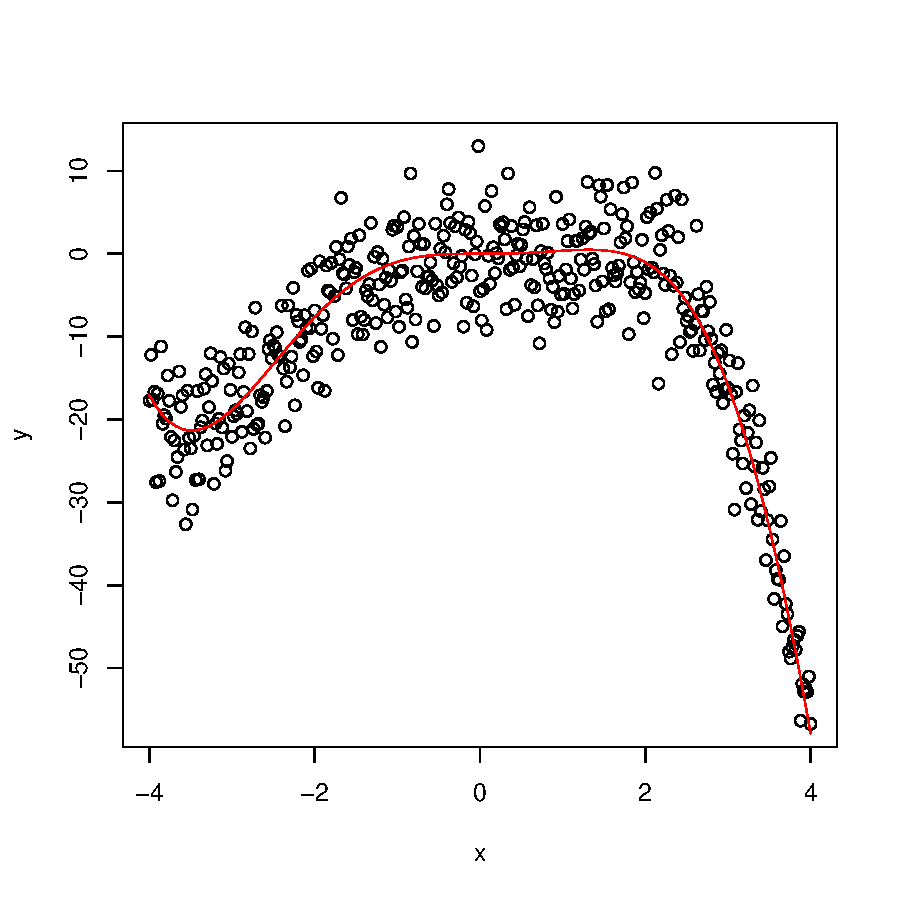
\includegraphics{week4-001}

\end{solution}
\item Try normal kernel smoothing with different bandwidths on “datasmooth.txt”.
\begin{solution}
Let us first import the Kernel Smoothing package
\begin{Schunk}
\begin{Sinput}
> library(KernSmooth)
> x <- data$x
> y <- data$y
> fit1 <- locpoly(x, y, kernel="normal", bandwidth=0.1)
> fit2 <- locpoly(x, y, kernel="normal", bandwidth=0.9)
> plot(data)
> lines(fit1, col = "red")
> lines(fit2, col = "green4")
\end{Sinput}
\end{Schunk}
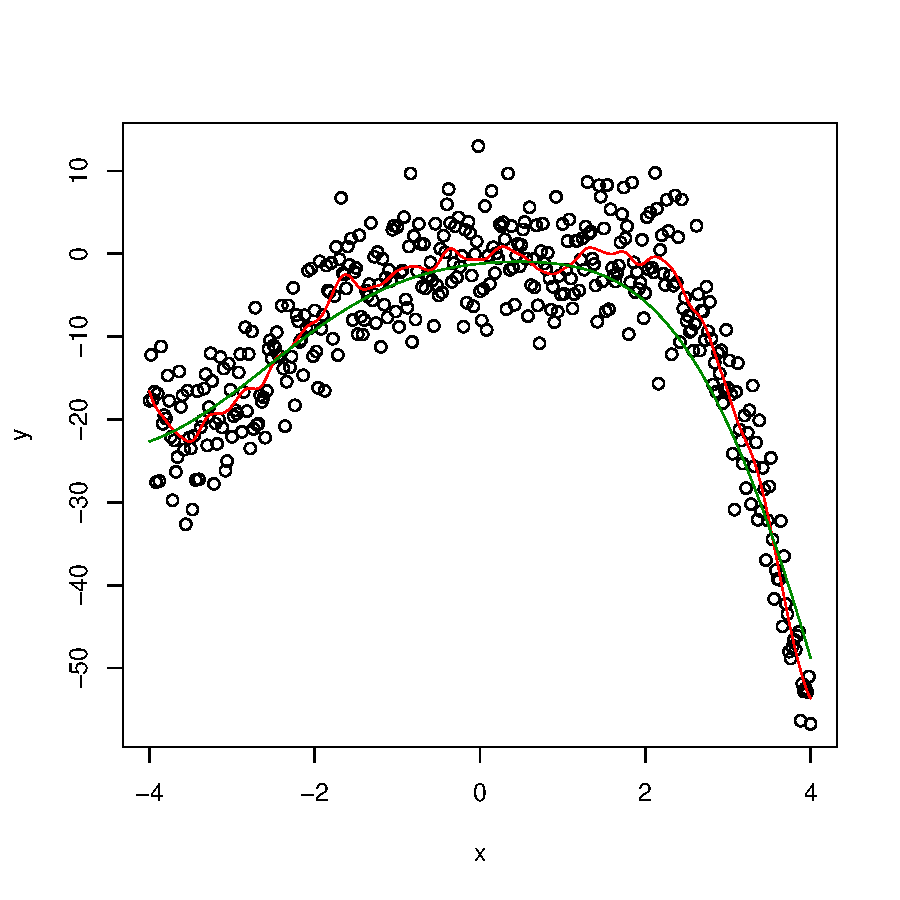
\includegraphics{week4-002}

\end{solution}
\item Apply cubic spline with different spars on “datasmooth.txt”. 
\begin{solution}
Let us make use of the R cubic spline;
\begin{Schunk}
\begin{Sinput}
> plot(data)
> cubicSpline1.fit <- smooth.spline(x=x, y=y, cv=FALSE, spar=0.5)
> cubicSpline2.fit <- smooth.spline(x=x, y=y, cv=FALSE, spar=1)
> cubicSpline3.fit <- smooth.spline(x=x, y=y, cv=TRUE)
> lines(cubicSpline1.fit, col = "blue")
> lines(cubicSpline2.fit, col = "green")
> lines(cubicSpline3.fit, col = "red")
> cubicSpline3.fit
\end{Sinput}
\begin{Soutput}
Call:
smooth.spline(x = x, y = y, cv = TRUE)

Smoothing Parameter  spar= 0.7581144  lambda= 0.0005645639 (13 iterations)
Equivalent Degrees of Freedom (Df): 11.27981
Penalized Criterion (RSS): 9036.802
PRESS(l.o.o. CV): 23.83662
\end{Soutput}
\end{Schunk}
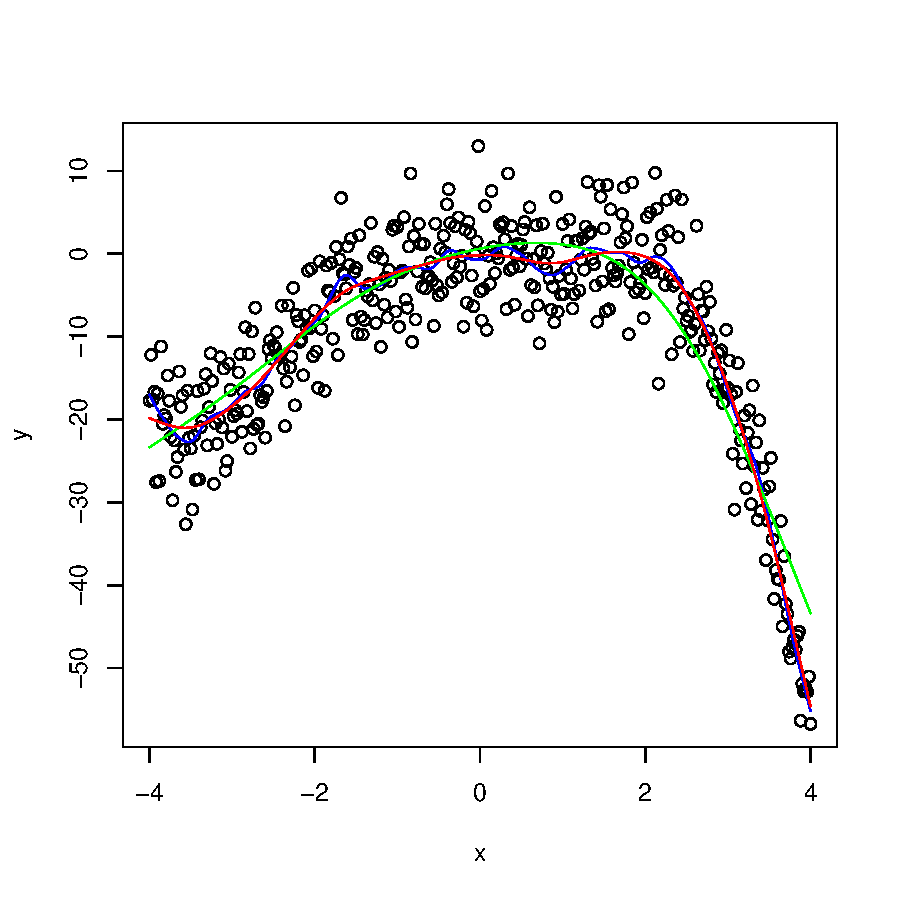
\includegraphics{week4-003}

\end{solution}
\item “newDatasmooth.txt” contains the <x, y> pairs generated from the same function.
Utilise this new dataset to estimate mean squared error and select best bandwidths
and spars for kernel smoother and cubic spline, respectively. 
\begin{solution}
Let us first import the new data set:
\begin{Schunk}
\begin{Sinput}
> newdata <- read.table("newDatasmooth.txt", header=TRUE, sep = "\t")
> head(newdata)
\end{Sinput}
\begin{Soutput}
      x         y
1 -4.00 -12.61164
2 -3.96 -15.17901
3 -3.92 -23.28943
4 -3.88 -20.42623
5 -3.84 -14.98288
6 -3.80 -22.82512
\end{Soutput}
\begin{Sinput}
> xn <- newdata$x
> yn <- newdata$y
> optimBw <- dpill(xn, yn)
> optimBw
\end{Sinput}
\begin{Soutput}
[1] 0.3034217
\end{Soutput}
\begin{Sinput}
> cubicSpline3.fit
\end{Sinput}
\begin{Soutput}
Call:
smooth.spline(x = x, y = y, cv = TRUE)

Smoothing Parameter  spar= 0.7581144  lambda= 0.0005645639 (13 iterations)
Equivalent Degrees of Freedom (Df): 11.27981
Penalized Criterion (RSS): 9036.802
PRESS(l.o.o. CV): 23.83662
\end{Soutput}
\end{Schunk}
Therefore the optimal bandwidth for the gaussian smoother is $0.303$ and the $0.76$ respectively. 
\end{solution}
\item Normal kernel smoother or cubic spline fits better to “datasmooth.txt”? 

\begin{solution}

Cubic spline is better in this case more closely matching the true curve.

\end{solution}
\end{enumerate}
\end{document}
